\section*{Questão 4}
% Enunciado
\noindent {\it Seja o sistema da Fig. \ref{fig:sist}. Considerando $G(s) =
\frac{2e^{-s}}{s+0.25}$, pede-se:

\begin{itemize}
    \item[a)] {\it projetar um controlador PI de forma que o desempenho do
              sistema em malha fechada não apresente sobre-sinal. Simule a 
              resposta no Matlab.}
    \item[b)] {\it Considerando o sistema com o controlador projetado no item a
              e considerando $G_d(s) = 1$, projetar um controlador feedforward 
              (realizável) e avaliar o desempenho do sistema completo utilizando
              o Matlab.}
\end{itemize}

\begin{figure}[htb]
\centering
    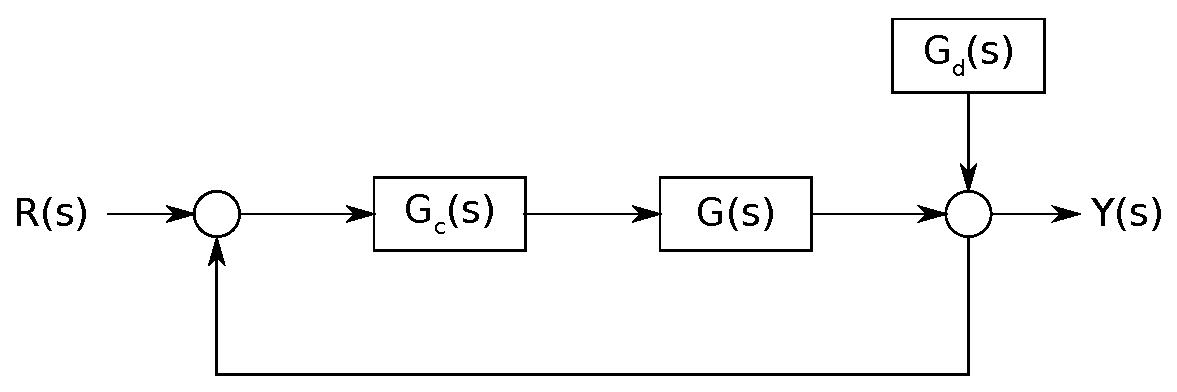
\includegraphics[width=0.65\textwidth]{imgs/questao4/sistema}
    \caption{Diagrama de blocos do sistema.}
    \label{fig:sist}
\end{figure}

\vspace{0.5cm}

\noindent{\bf Resolução:}

\vspace{0.25cm}

\noindent Bla bla bla
